\section{Results}
  \label{sec:results}

Our experiment revealed that the choice of coverage criterion did have an impact
on the performance of the test data generation tool. 
Figure~\ref{fig:crites} shows the results of the experiment for the BioSQL
schema.  The graph shows that runtime for certain criterions, such as AICC and AUCC increase faster than others, such as ANCC, APC, and
UCC.

\begin{figure}
\centering
  \centering
  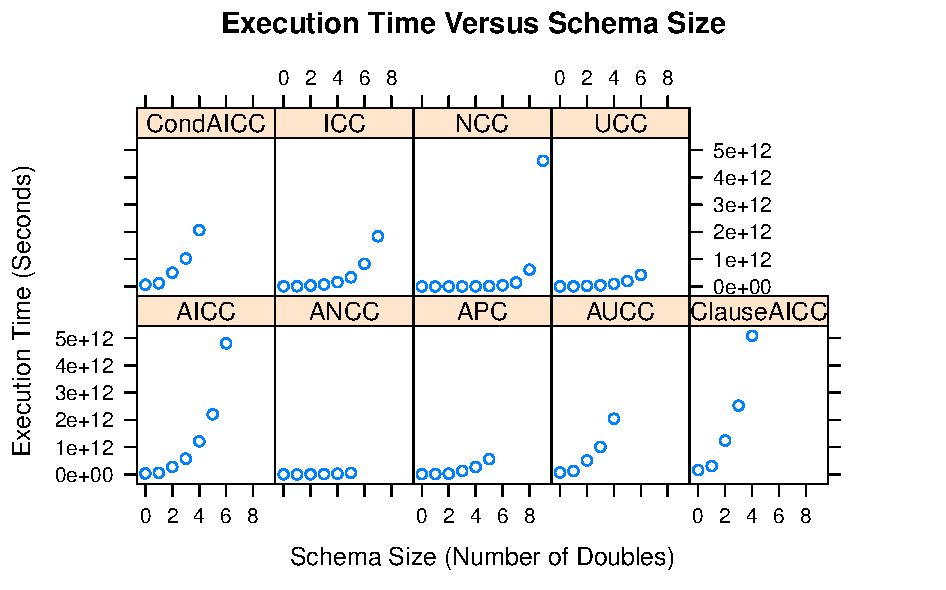
\includegraphics[width=1\linewidth]{../diagrams/TimevsSizeBioSqlDoubleAllonCriterion.pdf}
  \caption{Efficiency of SchemaAnalyst on BioSQL by coverage criterion.}
  \label{fig:crites}
  \vspace{-.15in} 
\end{figure}


\subsection*{Threats to Validity}

Our technique for doubling the number of check constraints on the schema
is simply to duplicate the existing check constraints. It is possible
that \textit{SchemaAnalyst} does less work processing these copied check
constraints than it would given unique check constraints. However,
doubling the check constraints in this way is an easy to implement,
semantically significant way of evaluating \textit{SchemaAnalyst}.

Additionally, since worst-case time is only apparent for large $n$, 
it is possible that the experiment terminated too quickly.  To guard 
against this problem, Algorithms~\ref{alg:convergence} and~\ref{alg:tuning}
were tested on various other algorithms with known worst-case complexities, and 
found to be reliable.
